\section*{Структура FILE}

\begin{lstlisting}
typedef struct _IO_FILE FILE;
struct _IO_FILE
{
  int _flags;		/* High-order word is _IO_MAGIC; rest is flags. */

  /* The following pointers correspond to the C++ streambuf protocol. */
  char *_IO_read_ptr;	/* Current read pointer */
  char *_IO_read_end;	/* End of get area. */
  char *_IO_read_base;	/* Start of putback+get area. */
  char *_IO_write_base;	/* Start of put area. */
  char *_IO_write_ptr;	/* Current put pointer. */
  char *_IO_write_end;	/* End of put area. */
  char *_IO_buf_base;	/* Start of reserve area. */
  char *_IO_buf_end;	/* End of reserve area. */

/* The following fields are used to support backing up and undo. */
  char *_IO_save_base; /* Pointer to start of non-current get area. */
  char *_IO_backup_base;  /* Pointer to first valid character of backup area */
  char *_IO_save_end; /* Pointer to end of non-current get area. */

  struct _IO_marker *_markers;

  struct _IO_FILE *_chain;

  int _fileno;
  int _flags2;
  __off_t _old_offset; /* This used to be _offset but it's too small.  */

/* 1+column number of pbase(); 0 is unknown. */
  unsigned short _cur_column;
  signed char _vtable_offset;
  char _shortbuf[1];

  _IO_lock_t *_lock;
  #ifdef _IO_USE_OLD_IO_FILE
};
\end{lstlisting}

\section*{Программа №1}

\begin{lstlisting}
#include <fcntl.h>
#include <stdio.h>

int main() {
  // have kernel open connection to file alphabet.txt
  int fd = open("alphabet.txt", O_RDONLY);
	
  // create two a C I/O buffered streams using the above connection
  FILE *fs1 = fdopen(fd, "r");
  char buff1[20];
  setvbuf(fs1, buff1, _IOFBF, 20);
	
  FILE *fs2 = fdopen(fd, "r");
  char buff2[20];
  setvbuf(fs2, buff2, _IOFBF, 20);
	
  // read a char & write it alternatingly from fs1 and fs2
  int flag1 = 1, flag2 = 2;
  while (flag1 == 1 || flag2 == 1) {
    char c;
		
    flag1 = fscanf(fs1, "%c", &c);
    if (flag1 == 1) fprintf(stdout, "%c", c);
		
    flag2 = fscanf(fs2, "%c", &c);
    if (flag2 == 1) fprintf(stdout, "%c", c);
  }
	
  return 0;
}
\end{lstlisting}
Результат работы программы:
\begin{figure}[H]
	\centering
	
\includegraphics[scale=0.8]{assets/p_1.png}
\end{figure}

Программа с дополнительным потоком:\newpage
\begin{lstlisting}
#include <fcntl.h>
#include <pthread.h>
#include <stdio.h>

void *thread_routine(void *fd) {
	int flag = 1;
	char c;
	
	FILE *fs = fdopen(*((int *)fd), "r");
	char buf[20];
	setvbuf(fs, buf, _IOFBF, 20);
	
	while (flag == 1) {
		flag = fscanf(fs, "%c", &c);
		if (flag == 1) {
			fprintf(stdout, "%c\n", c);
		}
	}
}

int main(void) {
	int fd = open("alphabet.txt", O_RDONLY);
	
	FILE *fs = fdopen(fd, "r");
	char buf[20];
	setvbuf(fs, buf, _IOFBF, 20);
	
	pthread_t thr_worker;
	
	pthread_create(&thr_worker, NULL, thread_routine, &fd);
	
	int flag = 1;
	char c;
	while (flag == 1) {
		flag = fscanf(fs, "%c", &c);
		if (flag == 1) {
			fprintf(stdout, "%c\n", c);
		}
	}
	pthread_join(thr_worker, NULL);
	return 0;
}
\end{lstlisting}

Результат работы программы:
\begin{figure}[H]
	\centering
	
\includegraphics[scale=0.8]{assets/p_1_thread.png}
\end{figure}

С помощью системного вызова open() создается дескриптор открытого только для чтения файла. Системный вызов open() возвращает индекс в массиве fd структуры files\_struct. fdopen() создает экземпляры структуры типа FILE(fs1 и fs2), которые ссылаются на дескриптор, созданный системным вызовом open.
Далее создаются буферы  buff1 и buff2 размером 20 байт. Для дескрипторов fs1 и fs2 помощью setbuv задаются соответствующие буферы и тип буферизации \_IOFBF(полная буферизация).

Далее fscanf() выполняется в цикле поочерёдно для fs1 и  fs2. Так как установлена полная буферизация, то при первом вызове fscanf() буфер будет заполнен полностью либо вплоть до конца файла, а f\_pos установится на следующий за последним записанным в буфер символ.

При первом вызове fscanf(fs1,"\%c",\&c); в буфер buff1 считаются первые 20 символов (abcdefghijklmnopqrst), в переменную c записывается, а затем выводится с помощью fprintf, символ 'a'. При первом вызове fscanf(fs2,"\%c",\&c);, в буфер buff2 считываются оставшиеся в файле символы – uvwxyz (в переменную с записывается символ 'u').  

Внутри цикла будут поочередно выводится символы из buff1 и buff2 до тех пор, пока символы в одном из буферов не закончатся. Тогда на экран будут последовательно выведены оставшиеся символы из другого буфера. 

Связь структур:
\begin{figure}[H]
	\centering
	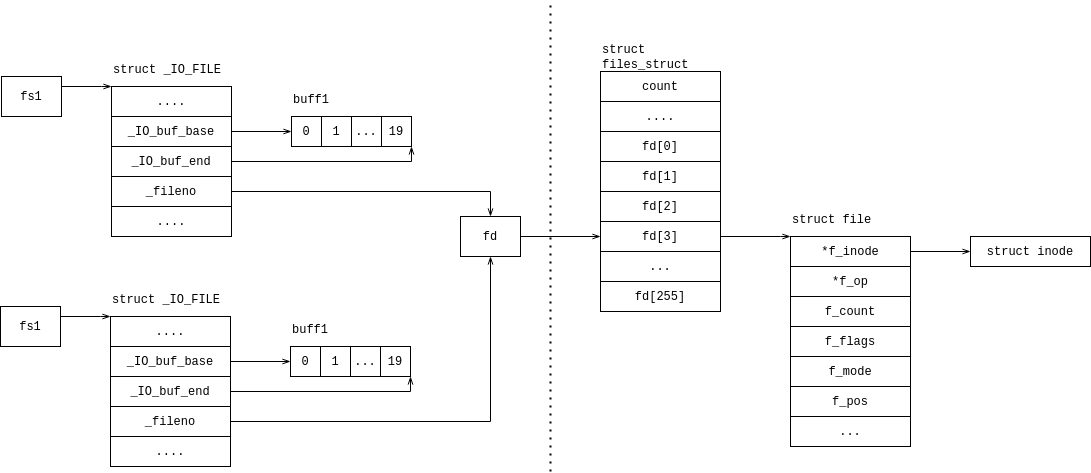
\includegraphics[scale=0.5]{assets/d_1.png}
\end{figure}

~\newline
\section*{Программа №2}
~\newline
\begin{lstlisting}
#include <fcntl.h>
#include <unistd.h>

int main() {
  int fd1 = open("alphabet.txt", O_RDONLY);
  int fd2 = open("alphabet.txt", O_RDONLY);

  char c;

  while (read(fd1, &c, 1) == 1 && read(fd2, &c, 1) == 1) {
    write(1, &c, 1);
    write(1, &c, 1);
  }

  return 0;
}
\end{lstlisting}
Результат работы программы:
\begin{figure}[H]
	\centering
	
\includegraphics[scale=0.8]{assets/p_2.png}
\end{figure}

Программа с дополнительным потоком:
\begin{lstlisting}
#include <fcntl.h>
#include <pthread.h>
#include <stdio.h>
#include <unistd.h>

pthread_mutex_t mux;

void *thread_routine(void *arg) {
  int fd = *((int *)arg);
  
  int flag = 1;
  char c;
  
  pthread_mutex_lock(&mux);
  while (flag == 1) {
    flag = read(fd, &c, 1);
    if (flag == 1) write(1, &c, 1);
  }
  pthread_mutex_unlock(&mux);
}

int main() {
  int fd1 = open("alphabet.txt", O_RDONLY);
  int fd2 = open("alphabet.txt", O_RDONLY);
  
  pthread_t thr_worker;
  
  if (pthread_mutex_init(&mux, NULL) != 0) {
    printf("can't pthread_mutex_init.\n");
    return 1;
  }
  
  pthread_create(&thr_worker, NULL, thread_routine, &fd1);
  
  int flag = 1;
  char c;
  
  pthread_mutex_lock(&mux);
  while (flag == 1) {
    flag = read(fd2, &c, 1);
    if (flag == 1) write(1, &c, 1);
  }
  pthread_mutex_unlock(&mux);
  
  pthread_join(thr_worker, NULL);
  
  return 0;
}
\end{lstlisting}
Результат работы программы:
\begin{figure}[H]
	\centering
	
\includegraphics[scale=0.8]{assets/p_2_thread.png}
\end{figure}

В программе один и тот же файл открыт 2 раза для чтения.  При вызове системного вызова open() создается дескриптор файла в системной таблице файлов, открытых процессом и запись в системной таблице открытых  файлов.  Так как в данном случае файл открывается 2 раза, то в таблице открытых процессом файлов будет 2 дескриптора и каждый такой дескриптор имеет собственный f\_pos. По этой причине чтение становится независимым --  при вызове read() для обоих дескрипторов по очереди, оба указателя проходят по всем позициям файла, и каждый символ считывается и выводится по два раза. 
Несмотря на то, что существует 2 дескриптора открытого файла, открывается один и тот же файл, т.е. inode один и тот же.

Связь структур:
\begin{figure}[H]
	\centering
	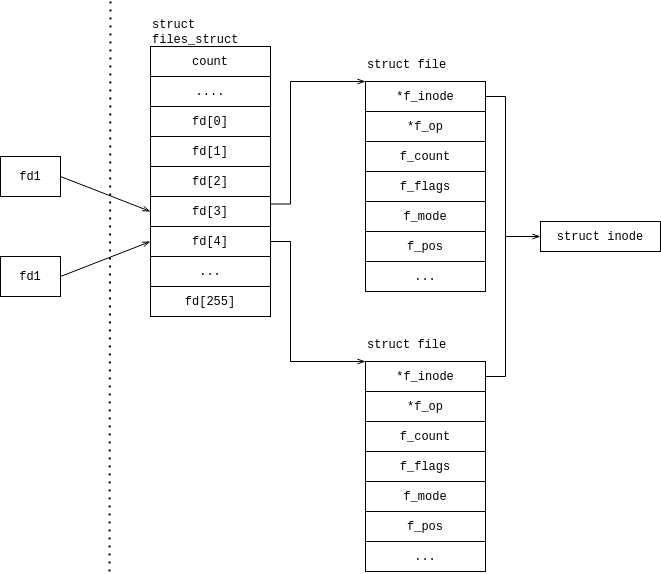
\includegraphics[scale=0.7]{assets/d_2.png}
\end{figure}


~\newline
\textsc{\huge Программа №3} \\
~\newline
Написать программу, которая открывает один и тот же файл два раза с использованием библиотечной функции fopen(). Для этого объявляются два файловых дескриптора. В цикле записать в файл буквы латинского алфавита поочередно передавая функции fprintf() то первый дескриптор, то – второй.
Результат прокомментировать.

\begin{lstlisting}
#include <fcntl.h>
#include <stdio.h>
#include <unistd.h>
int main() {
  FILE *f1 = fopen("out.txt", "w");
  FILE *f2 = fopen("out.txt", "w");
  for (char letr = 'a'; letr < '{'; letr++) {
    letr % 2 ? fprintf(f1, "%c", letr) : fprintf(f2, "%c", letr);
  }
  fclose(f2);
  fclose(f1);
  return 0;
}
\end{lstlisting}
Результат работы программы:
\begin{figure}[H]
	\centering
	
\includegraphics[scale=0.8]{assets/p_3.png}
\end{figure}
Файл out.txt открывается функцией fopen() на запись дважды. Создается два дескриптора открытых файлов, две независимые позиции, но с одним и тем же inode. Функция fprintf() (функция записи в файл) самостоятельно создаёт буфер, в который заносимая в файл информация первоначально и помещается. Из буфера информация переписывается в результате трех действий:
\begin{enumerate}
	\item Информация из буфера записывается в файл когда буфер полон. В этом случае содержимое буфера автоматически переписывается в файл.
	\item Если вызван fflush - принудительная запись содержимого в файл.
	\item Если вызван fclose.
\end{enumerate}
В данном случае запись в файл происходит в результате вызова функции fclose. При вызове fclose() для fs1 буфер для fs1 записывается в файл. При вызове fclose() для fs2, все содержимое файла очищается, а в файл записывается содержимое буфера для fs2. В итоге произошла утеря данных, в файле окажется только содержимое буфера для fs2. \\
\textbf{Решение.} Необходимо использовать open() с флагом O\_APPEND. Если этот флаг установлен, то каждой операции добавления гарантируется неделимость. \\
Программа с дополнительным потоком:\newpage
\begin{lstlisting}
#include <fcntl.h>
#include <pthread.h>
#include <stdio.h>
#include <sys/stat.h>
#include <unistd.h>

struct stat statbuf;

void *thread_routine() {
  FILE *f2 = fopen("out.txt", "w");
  stat("out.txt", &statbuf);
  printf("open for fs2: inode  = %ld, buffsize = %ld blocksize= %ld\n",
         (long int)statbuf.st_ino, (long int)statbuf.st_size,
         (long int)statbuf.st_blksize);
  for (char letr = 'a'; letr < '{'; letr += 2) fprintf(f2, "%c", letr);
  fclose(f2);
  stat("out.txt", &statbuf);
  printf("close for fs2: inode  = %ld, buffsize = %ld blocksize= %ld\n",
         (long int)statbuf.st_ino, (long int)statbuf.st_size,
         (long int)statbuf.st_blksize);
}

int main() {
  FILE *f1 = fopen("out.txt", "w");
  stat("out.txt", &statbuf);
  printf("open for fs1: inode  = %ld, buffsize = %ld blocksize= %ld\n",
         (long int)statbuf.st_ino, (long int)statbuf.st_size,
         (long int)statbuf.st_blksize);

  pthread_t thr_worker;
  pthread_create(&thr_worker, NULL, thread_routine, f1);
  pthread_join(thr_worker, NULL);

  for (char letr = 'a'; letr < '{'; letr += 2) fprintf(f1, "%c", letr);

  fclose(f1);
  stat("out.txt", &statbuf);
  printf("close for fs2: inode  = %ld, buffsize = %ld blocksize= %ld\n",
         (long int)statbuf.st_ino, (long int)statbuf.st_size,
         (long int)statbuf.st_blksize);

  return 0;
}
\end{lstlisting}
Результат работы программы:
\begin{figure}[H]
	\centering
	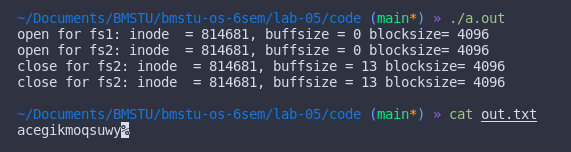
\includegraphics[scale=0.8]{assets/d_3_thread.png}
\end{figure}

Связь структур:
\begin{figure}[H]
	\centering
	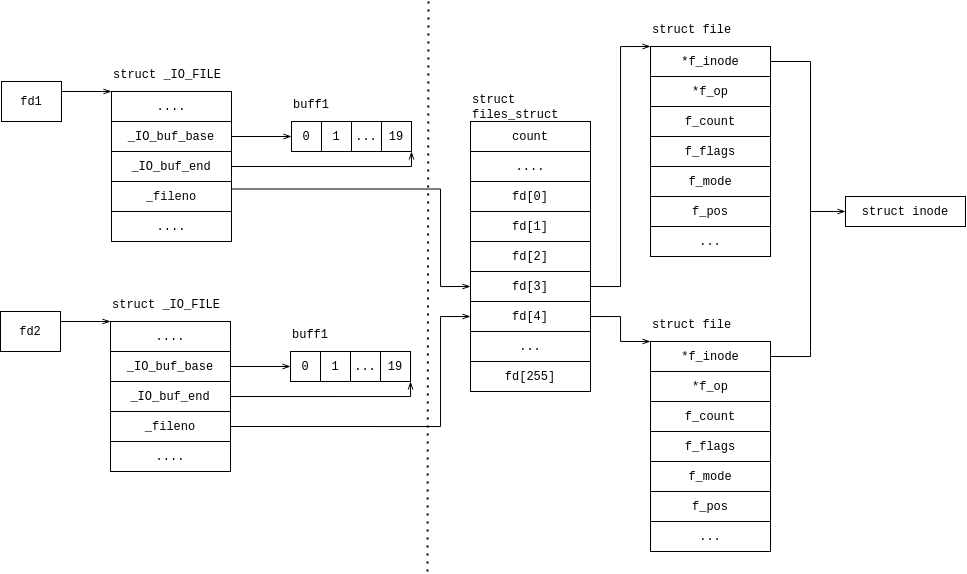
\includegraphics[scale=0.55]{assets/d_3.png}
\end{figure}